\section{Planknoten und Äquivalenzklassen}

Die unterschiedlichen Pläne werden in diesem Protypen als Äquivalenzklassen und Planknoten implementiert. Die Relationen werden mit Hilfe von Bitvektoren dargestellt. Im Folgenden wird auf die genaue Implementierung von Bitvektoren, Äquivalenzklassen und Planknoten eingegangen.

\subsection{Repräsentation von Relationen}
\label{sec:Bitvector}

Die einzelnen Relationen werden mit Hilfe eines Bitvektors dargestellt. Jeder Basis-Relation - sie repräsentiert eine physische Relation - ist eine ID zugeordnet. Eine Basis-Relation wird in diesem Prototypen mit Hilfe eines auf \texttt{TRUE} gesetzten Bits in einem Bitvektor repräsentiert. Auch mehrere Relationen können durch einen Bitvektor abgebildet werden dazu werden mehrere Bits auf \texttt{TRUE} gesetzt.

\subsubsection{Implementierung}

Als Basis für die Implementierung dient ein Bitvektor. Ein Bitvektor sind mehrere Bits, die entweder \texttt{TRUE} also \texttt{1} oder \texttt{FALSE} also \texttt{0} sein können. Ist das n-te Bit eines Bitvektors gesetzt, so repräsentiert dieses Bit die n-te Relation. Beispielsweise bezeichnet der Bitvektor \texttt{010000000} die Relation mit der ID \texttt{1}. Mit Hilfe des Bitvektors können auch mehrere Relationen gespeichert werden \texttt{01010000000} bezeichnet folglich die Relation mit dem Name \texttt{1} und die Relation mit der ID \texttt{3}. Für die durchgeführten Berechnungen ist es nicht notwendig, dass eine Relation mit ihrem tatsächlichen Namen bekannt ist. Es reicht eine Bezeichnung mit Hilfe von Nummern aus.

Vorteil für die Verwendung von Bitvektoren ist, dass einfach Mengenoperationen durchgeführt werden können. So kann einfach geprüft werden, ob Äquivalenzklassen gemeinsame JOIN Kanten besitzen oder neue Relationen einer Äquivalenzklasse hinzugefügt werden. (vgl. Abb. \ref{Bitvector}) Dies ist besonders effizient, da nur Bits und keine komplexen Objekte wie Strings verarbeitet werden müssen.



\begin{figure}[ht]
  \centering
  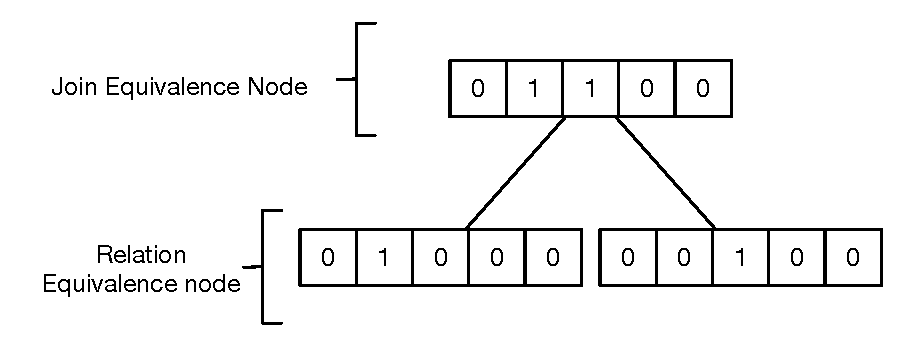
\includegraphics{04_Implementierung/00_media/Bitvector.pdf}
  \caption{Bitvekotren als Repräsentation von Relationen oder Joins}
  \label{Bitvektor}
\end{figure}


Die konkrete Erzeugung von Bitvektoren zu repräsentation von Relationen entsteht bei der Erstellung neuer Pläne bzgl. Äquivalenzklassen. Bezeichnet eine Äquivalenzklasse nur eine Basis-Relation so ist ihr Bitevektor \texttt{\_relations} auf nur einen Wert gesetzt. Wird einer Äuqivalenzklasse ein Planknoten hinzugefügt, wird die Variable \texttt{\_relations} mit den Relationen, die links bzw. rechts an einem Planknoten hängen, angereichert.



\subsubsection{Erweiterbarkeit}
Die Implementierung des Bitvektors erlaubt es mit Hilfe eines Templateparameters die Länge des Bitevektors anzupassen.



\subsection{Planknoten und Äquivalenzklassen}




\begin{figure}[ht]
  \centering
  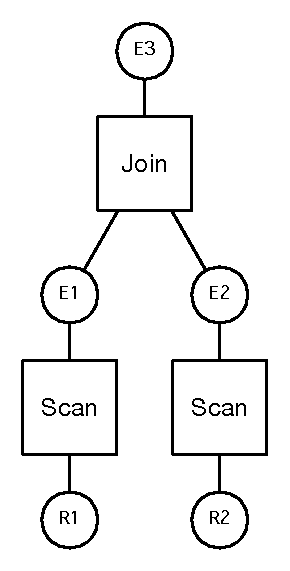
\includegraphics{04_Implementierung/00_media/JoinScan.pdf}
  \caption{Planknoten und Äquivalenzklassen}
  \label{PlanAequi}
\end{figure}

Die Datenstruktur in der Pläne gespeichert sind, sind sowohl \texttt{Plan\-Node} und \texttt{Equi\-valence\-Classes}. Einem Planknoten ist ein Operator zugewiesen. Beispielsweise \texttt{JOIN} oder \texttt{SCAN}. In \texttt{Equi\-valence\-Class} werden mehrere Pläne gespeichert, die alle semantisch gleich sind. Ein einfaches Beispiel ist in Abbildung \ref{PlanAequi} zu finden. Ein einfacher Plan bestehend aus einem Join und zwei Scans ist zu sehen. Der oberste Knoten \texttt{E3} ist eine Äquivalenzklasse. In ihr findet sich der erste Planknoten ein Join. Der Join hat zwei Seiten, eine linke und eine rechte. Beide Seiten sind mit einer Äquivalenzklasse verbunden \texttt{E1} resp. \texttt{E2}, die jeweils einen Scan beinhalten, der die Basis-Relationen \texttt{R1} bzw. \texttt{R2} einliest. Die beiden Basis-Relationen sind ebenso wie die Äquivalenzklassen als \texttt{Equi\-valence\-Class} im System abgelegt.




\subsubsection{Implementierung von Äquivalenzklassen}

\begin{figure}[ht]
  \centering
  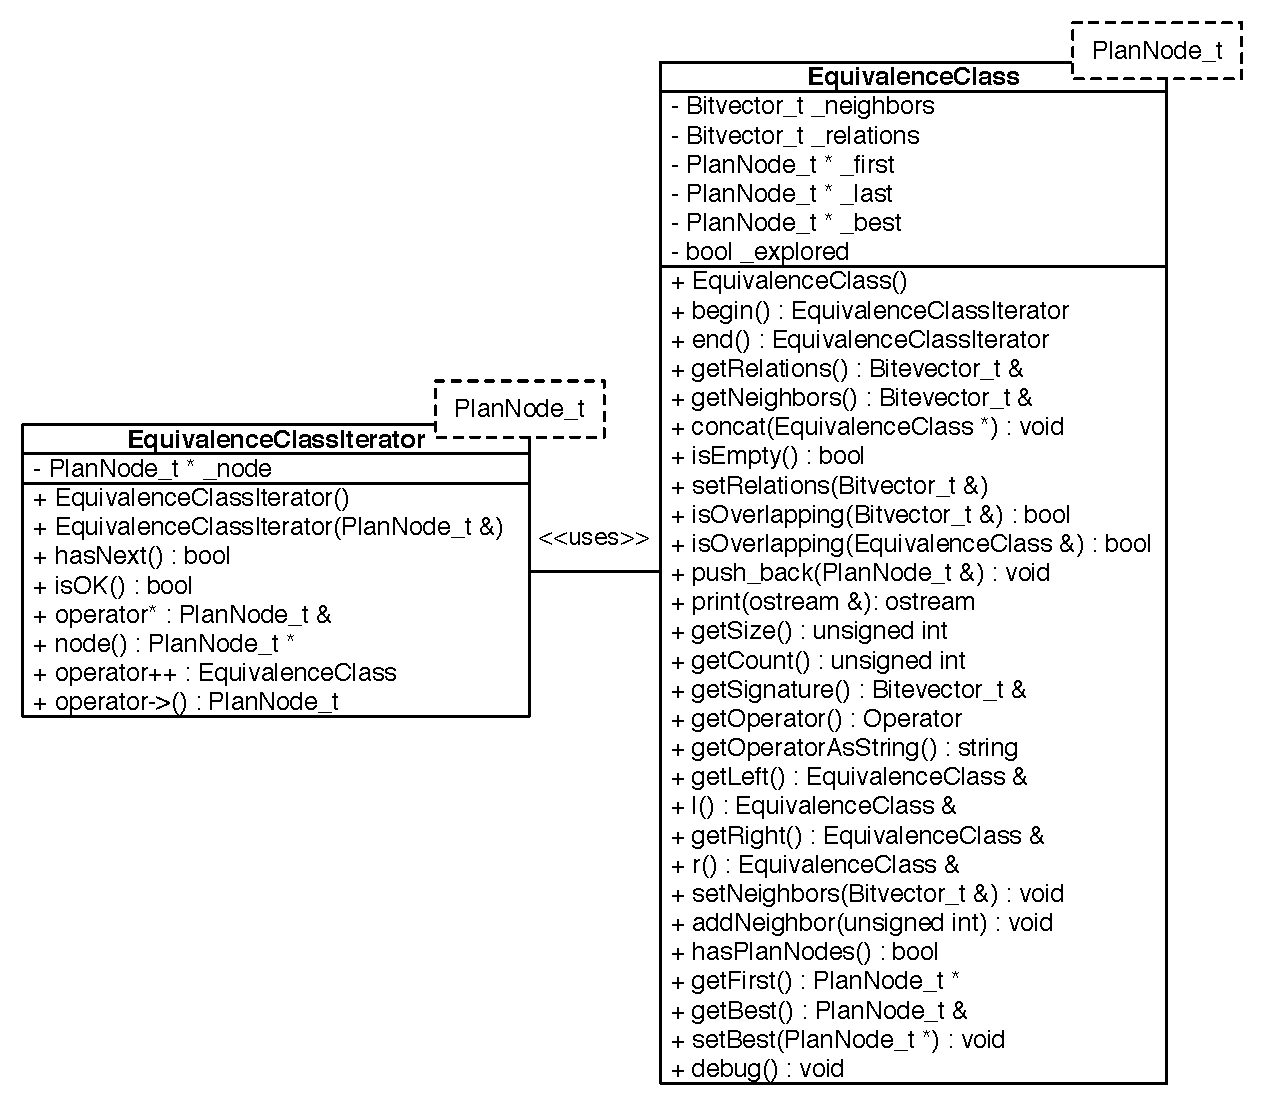
\includegraphics[width=1\textwidth]{04_Implementierung/00_media/ClassEquivalenceClass.pdf}
  \caption{Klassendiagramm: Äquivalenzklasse}
  \label{ClassEquivalenceClass}
\end{figure}


Wie bereits beschrieben, werden semantisch gleiche Planknoten in Äquivalenzklassen gespeichert und Basis-Relationen durch Äquivalenzklassen repräsentiert. Die konkrete Implementierung der Äquivalenzklasse ist in Abb. \ref{ClassEquivalenceClass} zu erkennen.

Bevor ein Plan einer Äquivalenzklasse zugeordnet werden kann oder eine Relation repräsentiert werden kann, muss die Äquivalenzklasse instantiiert werden. Bei der Instantiierung befinden sich noch keine Informationen über Planknoten oder Relationen in der Äquivalenzklasse. Die Variablen \texttt{\_first}, \texttt{\_last} und \texttt{\_best}, die den ersten, den letzten und den besten Plan anzeigen, sind auf \texttt{NULL} gesetzt. Die Bitvektoren \texttt{\_relations} und \texttt{\_neighbors} sind leer und repräsentieren noch keine Relationen. Auch die boolean variable \texttt{\_explored}, die anzeigt, ob eine Äquivalenzklasse schon vollständig erforscht ist, ist auf falsch gesetzt.


Von diesem Startpunkt aus, kann eine Äquivalenzklasse zwei Wege einschlagen: entweder eine Menge von Plänen speichern oder Basis-Relationen speichern. 

Wird eine Basis-Relation gespeichert, so kann mit der Methode \texttt{setRelations( Bitvector\_t \& )} eine Bitevektor übergeben werden. Die Nachbarschaft einer \texttt{Equi\-valence\-Class} kann mit der Methode \texttt{setNeighbors( Bitvector\_t \& )} festgelegt werden. Als Nachbarschaft werden die Knoten bezeichnet, mit denen eine Join-Kante besteht.




Falls die Äquivalenzklasse mehrere Pläne speichert, kann auf einen Knoten mit Hilfe der Methode \texttt{push\_back( PlanNode\_t \& )} ein Planknoten angehängt werden. Zuerst wird geprüft, ob bereits ein Planknoten vorhanden ist. Falls das nicht der Fall ist, wird der Knoten als erster, \texttt{\_first}, und als letzter, \texttt{\_last}, Knoten in der Äquivalenzklasse festgelegt. Im selben Schritt wird von dem Planknoten die Nachbar- und die vorkommenden Relationen in den dafür vorgesehenen Bitevektoren gespeichert. Falls ein Knoten schon vorhanden ist, wird auf dem letzten Knoten die Methode \texttt{setNext( PlanNode\_t \& )} aufgerufen. Diese hängt an einen Planknoten einen weiteren an. Die konkrete Implementierung hängt vom jeweils verwendeteten Planknoten ab. Die exakte Implementierung ist im Code-Beispiel \ref{listing:Push-Back} zu sehen.

\lstinputlisting[caption=C++: EquivalenceClass push\_back, label=listing:Push-Back]{04_Implementierung/00_media/Push_back.h}

Eine weitere Möglichkeit Pläne an eine Äquivalenzklasse anzuhängen ist die Methode \texttt{concat(EquivalenceClass *)} Eine andere Äuqivalenzklasse kann übergeben werden und wird automatisch an die bestehende Klasse angehängt. So können zwei Äquivalenzklassen kombiniert werden.



Ein weiterer wichtiger Teil, der gesondert hervorgehoben werden muss, ist die Methode \texttt{isOverlapping( Bitevector\_t \& )} Die Methode wird  verwendet um zu prüfen, ob die Nachbarn einer Äquivalenzklasse in einem gegebenen Bitvektor vorkommen. Repräsentiert eine Äquivalenzklasse beispielsweise die Relation 1,2,3 und hat die Nachbarn 4, 5 und 6., so gibt die Methode \texttt{isOverlapping true} zurück, falls der Eingabe-Bitvektor 4, 5 und/oder 6 enthält. Dieser Zustand wird im weiteren auch als überlappend bezeichnet und wird genutzt um zu prüfen, ob eine Regel anwendbar ist.

Ebenfalls ist es notwendig, über die in einer Äquivalenzklasse gespeicherten Pläne zu iterieren. Eine Äuqivalenzklasse kann sich wie in Abb. \ref{EquivalenceClassList}. Die Äquivalenzklasse zeigt mit dem Zeiger \texttt{\_first} auf den ersten Planknoten. Dieser Zeit auf den nächsten Planknoten. Auf den letzten Planknoten wird von der Äuqivalenzklasse mit dem Zeiger \texttt{\_last} gezeigt. Der beste Plan wird mit dem Zeiger \texttt{\_best} markiert. Bei der Iteration über die Pläne einer Äquivalenzklasse kommt die Methode \texttt{begin()} zum Einsatz, die einen Iterator für den ersten Plan zurückliefert. Wird die Methode \texttt{node()} auf den Iterator angewendet, wird der jeweilige Planknoten zurückgeliefert. Neben der Methode für den ersten Knoten, lässt sich auch mit \texttt{last()} das letzte Element zurückliefern. So kann über die Menge der Planknoten iteriert werden.

\begin{figure}[ht]
  \centering
  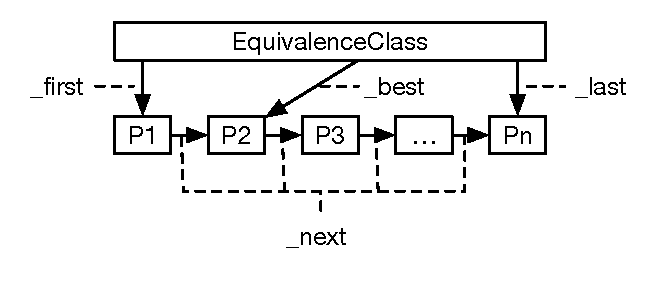
\includegraphics{04_Implementierung/00_media/EquivalenceClassList.pdf}
  \caption{Schematische Darstellung einer Äquivalenzklasse mit mehreren Planknoten}
  \label{EquivalenceClassList}
\end{figure}


\subsubsection{Implementierung von Planknoten}

\begin{figure}[ht]
  \centering
  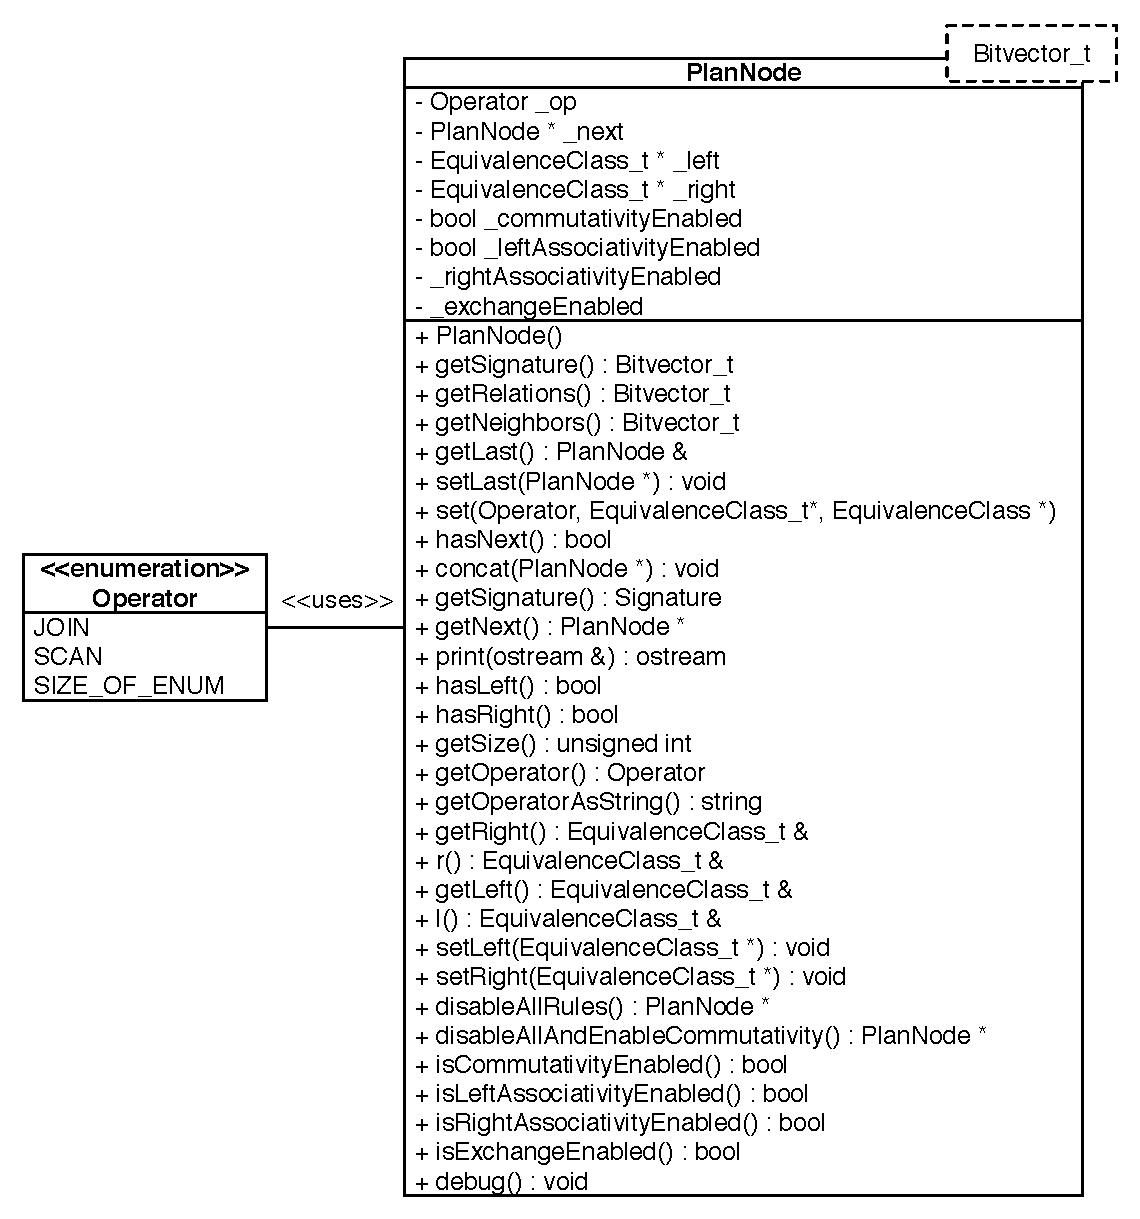
\includegraphics[width=\textwidth]{04_Implementierung/00_media/PlanNodeClass.pdf}
  \caption{Klassendiagramm: PlanNode}
  \label{PlanNodeClass}
\end{figure}

Wie bereits beschrieben, können Äuqivalenzklassen zur Speicherung von Plänen genutzt werden. Ein Planknoten repräsentiert eine Operation und kann bis zu zwei Äquivalenzklassen beinhalten. Wie in Abbildung \ref{PlanNodeClass} zu sehen, beinhaltet der Planknoten Zeiger auf einen linken und einen rechten Äquivalenzknoten, sowie einen Zeiger auf den nächsten Planknoten. Ebenso ist ein Operator Teil des Planknotens. Auch sind vier boolean Variablen vorhanden. \texttt{\_commutativity\-Enabaled}, \texttt{\_left\-Associativity\-Enabled},  \texttt{\_right\-Associativity\-Enabled},  \texttt{\_exchange\-Enabled}. Durch den Konstruktor werden die boolean Variablen auf \texttt{true} gesetzt und die Zeiger mit \texttt{NULL} initialisiert. Den Zeigern und dem Operator können später durch die Methode \texttt{set} mit konkreten Zeigern und einem Operator zugewiesen werden.



Der nächste Planknoten wird an den bestehenden Planknoten mittels der Methode \texttt{concat( PlanNode * )} angefügt.Falls der aktuelle Knoten nicht der letzte ist,kann mit der Methode contact (PlanNode *) zuerst zum letzten Knoten gesprungen werden und dort der neue Knoten eingefügt werden. 

Die Methoden \texttt{disable\-All\-Rules()} und \texttt{disable\-All\-And\-Enable\-Commutativity()} kommen bei der Verwendung des Regelsets \texttt{RS-B2} zum Einsatz. Nach Anwendung einer Regel wird so im Planknoten festgelegt, dass bestimmte Regeln nicht mehr auf einen Knoten angewendet werden dürfen. Um sicherzustellen, dass die Regeln nur \texttt{is\-Left\-Associativity\-Enabled()}, \texttt{is\-Right\-Associativity\-Enabled()} und \texttt{is\-Exchange\-Enabled()} geprüft, ob eine Regel zur Anwendung kommen darf.

Um die Äquivalenzklasse eines Planknotens zu erreichen ist es möglich mit der Methode \texttt{left()} bzw. \texttt{l()} einen Zeiger auf die entsprechende Klasse zu erhalten. Analog dazu können die Methoden \texttt{right()} bzw. \texttt{r()} verwendet werden. Mit den Methoden \texttt{has\-Left()} bzw. \texttt{has\-Right()} kann geprüft werden, ob ein Planknoten eine rechte bzw. linke Äquivalenzklasse besitzt. Diese Methoden sind insbesondere für die Implementierung von Regeln wichtig.


\subsubsection{Erweiterbarkeit}

Auch Planknoten und Äquivalenzklassen sind leicht erweiterbar. Auf der einen Seite ist es möglich die \texttt{Plan\-Node} vollkommen auszutauschen. Dies ist besonders einfach möglich, da die Äquivalenzklasse \texttt{PlanNode\_t} als Template-Parameter vorsieht und somit der Weg geebnet ist einen weiteren Knoten anzufügen. Neben dieser Erweiterung ist es ebenfalls denkbar, dass mehr als zwei Äquivalenzklassen einem Planknoten zugeordnet sind. 